\documentclass[11pt]{article}

\usepackage[utf8]{inputenc}
\usepackage[margin=1in]{geometry}
\usepackage[english]{babel}
\usepackage{tocloft}
\usepackage{amsmath}
\usepackage{amsfonts}
\usepackage{amssymb}
\usepackage[none]{hyphenat}
\usepackage{graphicx}
\usepackage{fancyhdr}
\usepackage{pdfpages}
\usepackage[font={small,it}]{caption}

\newcommand{\code}[1]{\texttt{#1}}


\parindent 0ex
\linespread{1.5}
\setlength{\headheight}{30pt}
\setcounter{tocdepth}{1}
\pagestyle{fancy}

\fancyhead{}
%\fancyfoot{}
\fancyhead[L]{\slshape \MakeUppercase{CROSS User Manual}}
\rhead{
\includegraphics[width=1cm, height=1cm]{cryogen.png}}

\begin{document}
	%insert pdf cover page
	
\includepdf[pages={-},offset=0mm 0mm, width=21.5cm, height=28cm]{Cover.pdf}

    \renewcommand{\cftsecleader}{\cftdotfill{\cftdotsep}} % TOC Dotted Lines
    \tableofcontents
    \thispagestyle{empty}
    \clearpage

	%\printglossary[title=Abbreviation]

    \setcounter{page}{1}

	\section{Introduction}
		\subsection{Intended Readership}
			This documented is intended for the users of the CROSS(Consensus-Ranking Organizational-Support System) application used to model Analytical Hierarchy Process used in this case to aid users in the process of deciding which projects to prioritize by evaluating the perks of all the projects against eachother. CROSS is developed by a computer science student at the North-West University, Zander Labuschagne.

		\subsection{Applicability}
			This user manual only applies to version 1.x of the CROSS application developed and maintained by Zander Labuschagne.

		\subsection{Purpose}
			The purpose of this document is to aid the users of the CROSS application so they can use it properly and as intended by the developers. This document hopes to clarify any misunderstandings its users might have.

		\subsection{Motivation \& Background}
			CROSS is developed as part of the Decision Support Systems II module for B.Sc. Computer Science \& Information Systems Honours students at the North-West University, Potchefstroom Campus. The goal of this project was to provide students with practical experience in any decision support model chosen by the student. It was expected of a student to develop a decision support application with a user friendly graphical user interface that demonstrates any decision support model chosen by the student that is at least to difficult for a second year computer science student to complete. This particular application was inspired by the original CROSS Excel system developed by Dr. Madjid Tavana who developed the system to aid NASA with their decision making in their projects \cite{tavana1996cross}. The original system developed by Dr. Tavana made use of specific criteria set by the people at NASA \cite{tavana2003cross}, this project generalized the idea to suit any type of projects.
	
	\section{User Guide}
		\subsection{Support}
			\subsubsection{Linux}
				This project was partly developed on a GNU/Linux system, more specifically Manjaro ArchLinux 17.03 - 17.05 KDE x86\_64 running Manjaro kernel version 4.13. Linux systems are fully supported and CROSS is expected to run flawless on these systems, but as the GPL 3.0 license states it is not guaranteed. Any bugs and inconsistencies may be reported to the developers and maintainers of this application, at least one of the developers aims to maintain this project for UNIX-like systems. A shell script named install.sh is provided which one can run to install the application on a Linux system. The installation adds an application entry to the applications menu or better known as a desktop entry for the application. Since a Java .jar file is provided one can run the .jar executable on Linux systems if Java Runtime Environment 1.8 or higher is installed, \textbf{very important: OpenJDK will not suffice!} But it is more convenient to do the installation and to use the application as intended. One can run the install with the terminal command \code{sudo sh install.sh}, if a permission error is encountered first enter the following command before installation: \code{sudo chmod +x install.sh}, this will add executable permission to the install script. To be able to read this document a PDF reader is required such as Okular.
				
			\subsubsection{macOS}
				This project was partly developed on a macOS 10.12.6 system but no dedicated installer or macOS executable(.app or .dmg) was made, there may be one in the future. macOS will be supported as far as possible, the developer does not have his own macOS system but currently has access to one at the university. Since a Java .jar file is provided one can run the .jar executable on a macOS system if Java Runtime Environment 1.8 or higher is installed. To be able to read this document a PDF reader is required such as Skim.

			\subsubsection{Windows}
				This application was never tested on a Windows platform and no support is provided for Windows systems. It is also very complicated to create an installer or portable .exe for Windows from a .jar executable and the little third party software that exists to make this process simpler is very expensive hence no Windows executable or installer. There is no guarantee that the developers will address any bugs or problems experienced on Windows systems but feedback is welcome just to keep record of what functions well. Since a Java .jar file is provided one can run the .jar executable on Windows systems if Java Runtime Environment 1.8 or higher is installed. To be able to read this document a PDF reader is required such as Adobe Reader.

		\subsection{Features Overview}
			This application does not have many features, it is simple and easy to use. 

			\subsubsection{Additional Features}
				The \code{Help} menu provides a button to open this document for help as well as an \code{About} form which displays information about the application as well as information about the developer(s). The \code{Look and Feel} menu provides additional look and feels or themes as some might call them, some people have different tastes than others which is why a light look and feel called \code{Midna} is included and two dark look and feels called \code{Midna Dark} and \code{Breath Dark}. The \code{Look and Feel} is not implemented properly yet and is thus not working, this is for future use.

			\subsubsection{Technical Features}
				The main programming langauage used is Java with Oracle Java Development Kit version 1.8. A JavaFX framework is used to display the graphical user interface, it includes .fxml files containing the graphical user interface layout, .css files containing information on how the graphical user interface looks and .java files containing code to execute instructions in order to provide functionality into the application. Some might not call this a feature but open source gives many advantages over closed source, this project is open source and available on GitHub, any feedback, criticism or pull requests are welcome.

	\section{Application Overview}
		This section explains how to use the application.\\
		
		The first window that is presented to the user is a welcome window that also prompts the user to enter the number of projects he or she wishes to evaluate against eachother. When done with the current window in any of the following steps the user may click \code{Continue} to proceed to the next window that will present the user with the next step.
		
		\subsection{Specifying the Criterions and their Weights}
			The second window presented to the user is the criterions specification window. This is where the user enters criterions chosen for the projects, the user then also specifies the criterion weight by adjusting the sliders accordingly for each criterion. This influences how important the criterion is when making the decisions. See \textit{figure \ref{fig:criterions}} for an example. Currently the number of criterions are limited to nine, this limitation will be taken care of in the future to have similiar functionality as the number of projects.
			
			\begin{figure}[!htb]
				\centering
				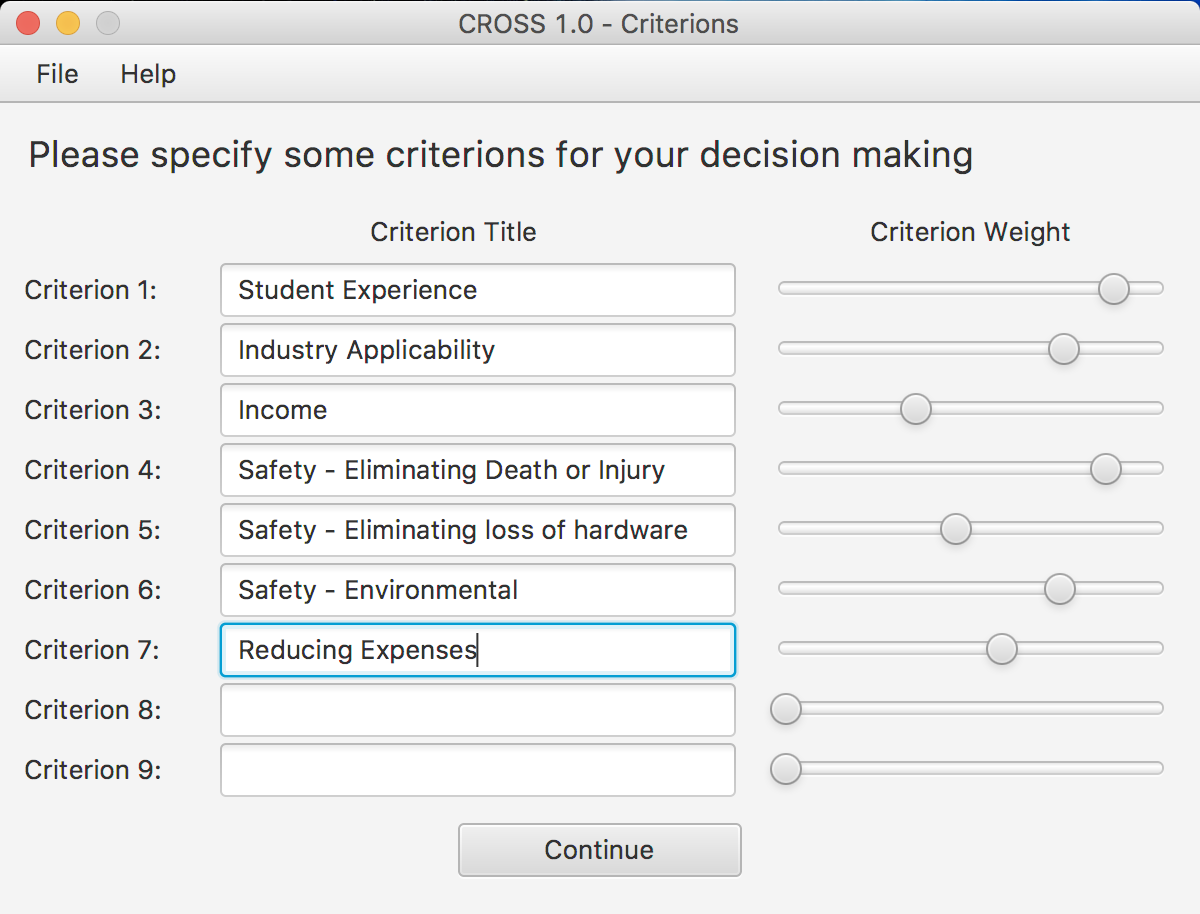
\includegraphics[scale=0.55]{criterions}
				\caption{Criterions Specification Window} % Figuur Naam
				\label{fig:criterions} % label om na figuur te verwys
			\end{figure}
			
		\subsection{Specifying Criterion Weights for each Project}
			The third window that is presented to the user, as is the few that will follow, are windows where the user specifies the criterion weights for each of the projects, one criterion per window. Windows will continue to present themselves until all the criterions are specifies for all the projects. An example of such a window can be seen in figure \textit{figure \ref{fig:criterion_iterator}}. On the first window the user will have to enter the project names, in this example only three projects are chosen to be evaluated. The project titles will then be automatically filled in the following windows, the user will only need to specify the criterion weight for each project by adjusting the slider accordingly.
			
			\begin{figure}[!htb]
				\centering
				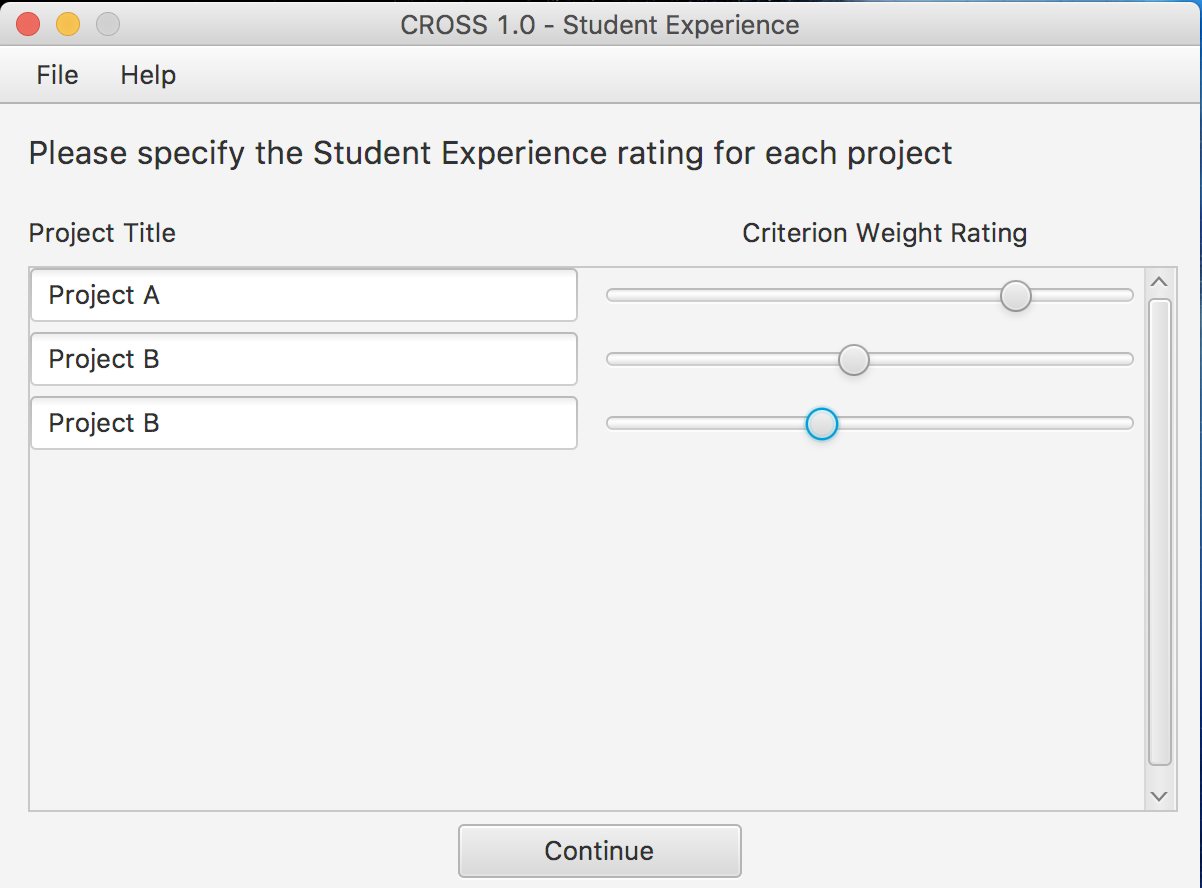
\includegraphics[scale=0.55]{criterion_iterator}
				\caption{Criterion Specification for each Project} % Figuur Naam
				\label{fig:criterion_iterator} % label om na figuur te verwys
			\end{figure}
			

		\subsection{Results}
			The final window that's presented to the user is the results window. This is where the user can see the ranking scores for each project, a project with a higher ranking score will provide more advantages according to the criterions specified by the user. A lower project ranking score represents a project that will not bring as many advantages. The consistency ration is a factor calculated and used to determine whether the user's decision making during the specification of the criterion weights is consistent \cite{taylor2004introduction}. The consitency ratio is calculated by using a \textit{random index}, this random index can be calculated in a number of ways, this project used Jos\'e Antonio Alonso's approach \cite{alonso2006consistency} to calculate a random index. See \textit{figure \ref{fig:results}}, the user may click the \code{Finish} button to end and close the application.
			
		\begin{figure}[!htb]
			\centering
			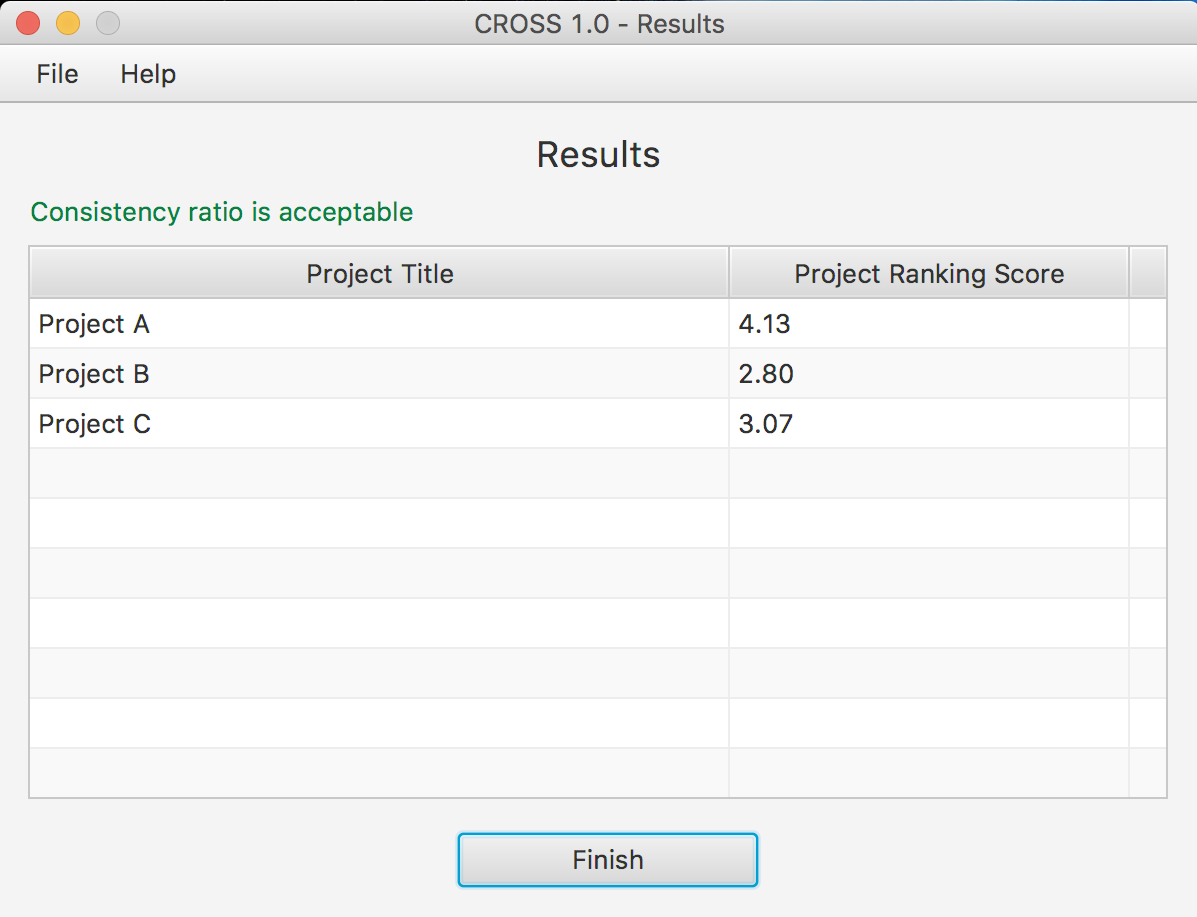
\includegraphics[scale=0.55]{results}
			\caption{Results Window} % Figuur Naam
			\label{fig:results} % label om na figuur te verwys
		\end{figure}
		
	\newpage
		

	\section{Acknowledgements}
		This project was developed and is being maintained with JetBrains IntelliJ IDEA Ultimate edition with a JetBrains student license. This documentation was compiled with \LaTeX. All non JavaFX icons are made by Madebyoliver from http://www.flaticon.com at http://www.flaticon.com/authors/madebyoliver and is licensed by Creative Commons BY 3.0. at http://creativecommons.org/licenses/by/3.0/. GitHub is used to do version control over this project since it is easily integrable with JetBrains IntelliJ. The decision support knowledge used in this project was gained from Introduction to management science by Bernard Taylor \cite{taylor2004introduction} and Prof. Hennie Kruger, the lecturer presenting the Decision Support Systems I and Decision Support Systems II module at the University of the North-West: Potchefstroom Campus. The inspiration of the project came from Prof. Madjid Tavana as mentioned earlier in section 1.4.

	\section{License}
		Copyright \textcopyright \space 2017 Zander Labuschagne. CROSS developed by Zander Labuschagne is free software: it may redistributed it and/or modified under the terms of the GNU General Public License version 3 as published by the Free Software Foundation. The full license can be viewed in the \code{LICENSE} file included.

    \section{Reflection}
		This section contains personal experiences and views from the developer's point of view while the project commenced.\\
		
		\subsection{Developer: Zander Labuschagne}
			I had little time to spare during the three days this project was being developed as I am also busy with my Honours project that has to be submitted within the next week, this is why there are some limitations on this application and why I did not include any theming as I usually do with my other projects. This is my fourth JavaFX application and every time I use it I make sure I learn something new. I have gained additional experience with CSS design though it was not implemented due to time retrictions. This project was my fourth project with GitHub integration, I can say with confidence that I have had no problems or hiccups during this project although I was working alone on this project. This was also the second time that I've used the Git Flow, it was not as good experience as it should be because it's not utilized to the full extent as it would when more than one developer use it. This project was a quick ``makeshift'' project derived from my Cryptogen encryption and decryption application.\\

			I would like to improve this application by not limiting the number of criterions and by adding CSS theming like I usually do. I would also like to add a green and red highlight to the table to highlight the good projects and the not so good projects. I have tried the highlighting but because of time constraints I did not continue to investigate why my code did not work.

		\newpage
		\bibliographystyle{plain}
		\bibliography{ref}
		\addcontentsline{toc}{section}{{}References}
		\thispagestyle{plain}
		\clearpage
\end{document}
